\documentclass[a4paper, 12pt]{report}

\usepackage{setspace}
\usepackage[italian]{babel}
% Useful packages
\usepackage{amsmath}
\usepackage{graphicx}
\usepackage{hyperref}
\usepackage{float}
\usepackage{mdframed}
\usepackage{comment}
\usepackage{makecell}
\usepackage{verbatim}

%diminuisco lo spazio sopra il capitolo
%-------------------------------------------
\usepackage{amssymb}
\usepackage{amsmath}
\usepackage{setspace}
\doublespacing 
\usepackage{etoolbox}
\makeatletter
\patchcmd{\@makechapterhead}{50\p@}{0pt}{}{}
\patchcmd{\@makeschapterhead}{50\p@}{0pt}{}{}
\makeatother
%-

\usepackage[letterpaper, left=1in, right=1in, top=1in, bottom=1in]{geometry}

\newenvironment{esempio}[2] [Esempio]
    { \begin{mdframed} \textbf{#1 #2}}
    {  \end{mdframed}}

\renewcommand\thesection{\arabic{chapter}.\arabic{section}} %le sezioni partono da 1


\title{Relazione di Sicurezza Informatica}
\author{Tassi Nicola \\ Matricola 719008}
\date{Laurea Magistrale in Ingegneria Informatica \\ A.A 2021 - 2022}


\begin{document}
\begin{spacing}{1.15}

\begin{titlepage}
    \begin{center}
        
\includegraphics[width=0.6\textwidth]{MainContent/img/intro/logo-Unibs.png}
        
        \LARGE
        \textbf{Sicurezza Informatica}
        
        \vspace{0.8cm}
        
        \LARGE
        Quantum Key Distribution (QKD)
            
        \vspace{2.5cm}
        
        Tassi Nicola \\ Matricola 719008
            
        \vfill
        
        \Large
        UNIVERSITÁ DEGLI STUDI DI BRESCIA\\
        Laurea Magistrale in Ingegneria Informatica\\
        A.A. 2021 - 2022
            
    \end{center}
\end{titlepage}

%Indice
\tableofcontents
\addcontentsline{toc}{chapter}{Introduzione}
\thispagestyle{empty}

\setcounter{page}{1}
\chapter*{Introduzione}
Negli ultimi tre decenni, la crittografia è diventata una componente indispensabile per la comunicazione tra individui distanti geograficamente. In un mondo così connesso, la capacità di individui, aziende e governi di comunicare in modo sicuro è fondamentale. 
Molti dei protocolli di comunicazione più importanti si basano principalmente su alcune funzionalità crittografiche tra cui: \textbf{crittografia a chiave pubblica}, \textbf{firme digitali} (funzioni hash) e \textbf{scambio di chiavi} (in questo documento tratteremo quest'ultimo). La crittografia a chiave pubblica attualmente in uso si basa su problemi che coinvolgono la fattorizzazione in numeri primi (RSA), i logaritmi discreti (Diffie-Hellman) e le curve ellittiche (ECC).
Anche se questi sembrano problemi diversi, in realtà sono tutti casi di un problema generale legato alla difficoltà di fattorizzazione in numeri primi.\\
Questo problema è difficile da risolvere, specialmente con algoritmi classici che hanno una complessità cosiddetta (sub)esponenziale. Ci vorrebbero anni per rompere l’attuale crittografia a chiave pubblica anche con il più potente dei computer, supponendo che il sistema sia implementato correttamente.\\
Nel 1994, Peter Shor ha dimostrato che i computer quantistici, una nuova tecnologia che sfrutta le proprietà fisiche della materia e dell'energia per eseguire calcoli, possono risolvere efficacemente ciascuno di questi problemi, rendendo così impotenti tutti i crittosistemi a chiave pubblica basati su tali presupposti \cite{shor_polynomial-time_1997}. In particolare, è stato dimostrato che l'algoritmo di Shor, se implementato su un calcolatore quantistico che utilizza un numero sufficiente di qbit, è in grado di risolvere il problema del logaritmo discreto e della fattorizzazione in numeri primi in tempo \textbf{polinomiale}, con tempi che crescono di poco al crescere della lunghezza delle chiavi crittografiche. Se mai verranno costruiti computer quantistici su larga scala, saranno in grado di violare molti dei crittosistemi a chiave pubblica attualmente in uso. Ciò comprometterebbe gravemente la riservatezza e l'integrità delle comunicazioni digitali su Internet e altrove. L'obiettivo della crittografia post-quantistica (\textit{post-quantum cryptography, quantum-resistant cryptography}) è sviluppare sistemi crittografici che siano sicuri sia contro i computer quantistici che classici e possano interagire con i protocolli e le reti di comunicazione esistenti. A questo proposito sono state ideate soluzioni che utilizzano elementi quantistici per arricchire e potenziare i protocolli già esistenti e l'esempio più noto è la distribuzione di chiavi quantistiche (QKD).
\chapter{Quantum Key Distribution}
Il Quantum Key Distribution (QKD) è un metodo di comunicazione sicuro che implementa un protocollo crittografico che coinvolge componenti di meccanica quantistica. Consente a due parti di produrre una chiave segreta casuale condivisa nota solo a loro, che può quindi essere utilizzata per criptare e decriptare i messaggi. Inoltre, invece di generare chiavi segrete una tantum utilizzate per più sessioni di comunicazione, i protocolli QKD possono fornire un flusso continuo di nuove chiavi segrete al fine di applicare la tecnica One Time Pad (OTP), la quale richiede che la chiave segreta non venga mai riutilizzata (venga utilizzata al massimo una volta).\\
Una proprietà importante e unica di questa tecnologia è il fatto che i due utenti in comunicazione possano rilevare la presenza di terze parti che cercano di acquisire informazioni sulla chiave. Ciò è reso possibile da una caratteristica fondamentale della meccanica quantistica: il processo di misurazione di un sistema quantistico, in generale, \textbf{disturba il sistema}. Una terza parte che cerca di intercettare la chiave deve in qualche modo misurarla, introducendo così anomalie rilevabili. Utilizzando sovrapposizioni quantistiche o l'\textbf{entanglement} quantistico e trasmettendo informazioni in stati quantistici, è possibile implementare un sistema di comunicazione che rilevi le intercettazioni. Se il livello di intercettazione è inferiore a una certa soglia, è possibile produrre una chiave di cui è garantita la sicurezza (ovvero, l'intercettatore non ha informazioni a riguardo), altrimenti non è possibile ottenere alcuna chiave sicura e la comunicazione viene interrotta.\\
Il protocollo QKD viene utilizzato solo per produrre e distribuire una chiave, non per trasmettere i dati del messaggio. Questa chiave può quindi essere utilizzata con qualsiasi algoritmo di crittografia scelto per criptare (e decriptare) un messaggio, che può quindi essere trasmesso su un canale di comunicazione standard \cite{shannon_communication_1949}.\\
La comunicazione quantistica implica la codifica delle informazioni in stati quantistici, o \textbf{qubit}, in contrasto con l'uso dei bit nella comunicazione classica. Di solito, i \textbf{fotoni} sono usati per rappresentare questi stati quantistici. Il QKD sfrutta alcune proprietà di questi stati quantistici per garantirne la sicurezza.\newpage
\noindent Esistono diversi approcci alla distribuzione delle chiavi quantistiche, ma possono essere divisi in due categorie principali a seconda della proprietà che sfruttano:
\begin{itemize}
    \item \textbf{Protocolli basati sulla preparazione e misurazione (PM):} Contrariamente alla fisica classica, l'atto della misurazione è parte integrante della meccanica quantistica. In generale, misurare uno stato quantistico sconosciuto cambia lo stato, in qualche modo. Questa è una conseguenza dell'indeterminatezza quantistica e può essere sfruttata per rilevare eventuali intercettazioni di comunicazione (che implicano necessariamente la misurazione) e, soprattutto, per calcolare la quantità di informazioni che è stata intercettata (es. protocolli BB84, B92).
    \item \textbf{Protocolli basati sull'entanglement (EB):} Gli stati quantistici di due (o più) oggetti separati possono essere "collegati" tra loro in modo tale da poter essere descritti da uno stato quantistico combinato, non come singoli oggetti. Questo è noto come \textbf{entanglement} e significa che, ad esempio, l'esecuzione di una misurazione su un oggetto influisce sull'altro. Se una coppia di oggetti quantistici collegati tra loro è condivisa tra due parti, chiunque intercetta uno dei due oggetti altera il sistema generale, rivelando la presenza della terza parte (e la quantità di informazioni che ha acquisito) (es. protocollo E91).
\end{itemize}

\noindent Come accennato in precedenza, i protocolli QKD non vengono utilizzati per crittografare i messaggi, ma vengono utilizzati per stabilire le chiavi segrete, che vengono poi utilizzate per criptare i messaggi. I messaggi crittografati vengono trasmessi attraverso i classici canali di comunicazione, cablati o wireless. Oltre al canale classico, i protocolli QKD richiedono un canale di comunicazione quantistico aggiuntivo per trasmettere gli stati quantistici che permettono poi di ricavare le chiavi segrete. Attualmente, il canale quantistico consiste in un canale a fibra ottica o wireless (aria).

\begin{figure}[H]
    \centering
    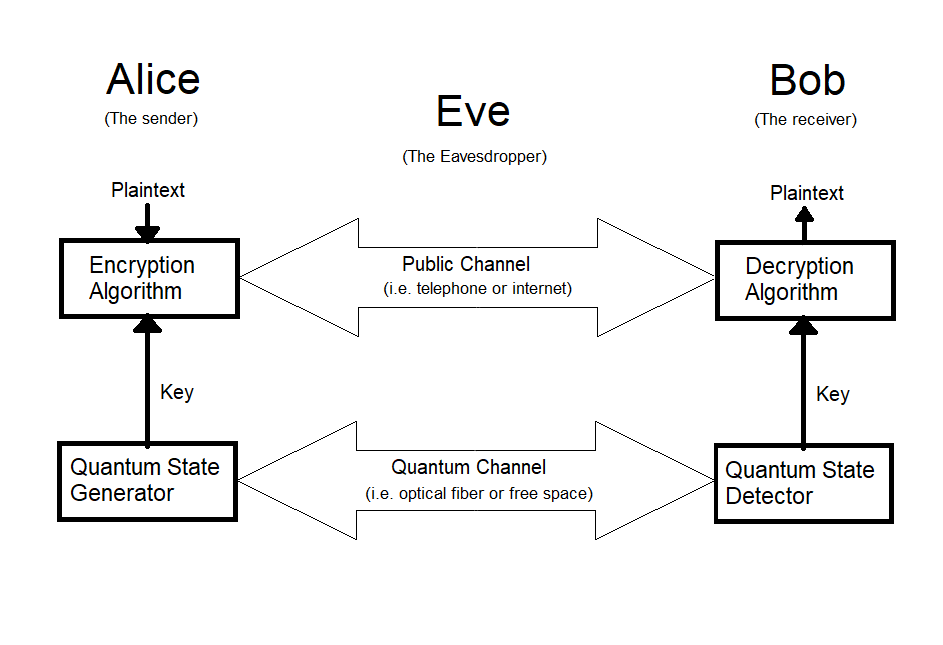
\includegraphics[width=0.85\textwidth]{MainContent/img/cap3/schema_QKD.png}
    \caption{QKD scheme}
    \label{fig:QKDscheme}
\end{figure}
\noindent
Come illustrato in Fig. \ref{fig:QKDscheme}, i protocolli QKD sono progettati per stabilire una chiave segreta solo tra una coppia di nodi mittente e destinatario, che sono collegati direttamente attraverso un canale quantistico senza alcun nodo intermedio. In quanto tali, sono protocolli peer-to-peer o point-to-point, sebbene il canale classico tra mittente e destinatario potrebbe non essere un collegamento diretto. Il canale classico viene utilizzato per trasmettere informazioni classiche, come il codice binario 1 o 0. D'altra parte, il canale quantistico viene utilizzato per trasmettere lo stato quantistico di una o più particelle (fotoni) \cite{yin_security_2016}.
Un’altra importante caratteristica operativa della QKD, quando viene utilizzata in sequenza per produrre chiavi di cifratura successive, come vedremo in seguito è la proprietà chiamata “forward-secrecy” delle chiavi: le chiavi successivamente scambiate con QKD sono indipendenti l’una dall’altra. Pertanto, la potenziale compromissione di una di esse non può portare alla compromissione delle altre. Questa è una caratteristica particolarmente apprezzabile sia per le reti ad elevata sicurezza, che per la memorizzazione a lungo termine dei dati (everlasting security).
Di seguito verrano descritti alcuni dei protocolli più noti, tra cui BB84, B92 e E91.
\newpage
\section{Protocollo BB84}
Questo protocollo, noto come BB84, prende il nome dai suoi inventori e dell'anno di pubblicazione \cite{bennett_quantum_2014}. Il mittente (tradizionalmente indicato come Alice) e il ricevitore (Bob) sono collegati da un canale di comunicazione quantistico che consente la trasmissione di stati quantistici. Nel caso dei fotoni, questo canale è generalmente una fibra ottica o semplicemente uno spazio libero. Inoltre, i due soggetti, comunicano tramite un canale pubblico classico, ad esempio tramite Internet. Il protocollo è progettato partendo dal presupposto che un attaccante (intercettatore denominato Eve) possa interferire in qualsiasi modo con il canale quantistico, mentre il canale classico deve essere autenticato e sicuro.\\
La sicurezza del protocollo deriva dalla codifica delle informazioni in stati non ortogonali. L'indeterminazione quantistica è causata dal fatto che questi stati non possono in generale essere misurati senza disturbare lo stato originale (Teorema di non clonazione). BB84 utilizza due coppie di stati, ciascuna coppia è coniugata all'altra e i due stati all'interno di una coppia sono ortogonali tra loro. Le coppie di stati di polarizzazione comunemente utilizzate sono:
\begin{itemize}
    \item La base rettilinea: verticale (0°) e orizzontale (90°)
    \item La base diagonale: 45° e 135°
\end{itemize}

Il primo passo è la trasmissione dei fotoni, Alice crea un bit casuale (0 o 1) e seleziona casualmente una delle sue due basi (rettangolare o diagonale). In seguito prepara uno stato di polarizzazione del fotone a seconda sia del valore del bit che della base, come mostrato nella Tabella \ref{tab:codifica_bit}. Quindi, ad esempio, uno 0 è codificato in base rettilinea (+) come stato di polarizzazione verticale e un 1 è codificato in base diagonale (x) come stato di 135°. Alice trasmette a Bob un singolo fotone nello stato predeterminato utilizzando il canale quantistico. Questo processo viene quindi ripetuto per ogni bit che Alice vuole inviare, registrando lo stato, la base e il tempo di trasmissione di ogni fotone.

\begin{table}[H]
\centering
    \begin{tabular}{|c|c|c|}
    \hline
    Basis & 0 & 1\\
    \hline
    $+$ & $\uparrow$ & $\rightarrow$\\
    \hline
    $\times$ & $\nearrow$ & $\searrow$\\
    \hline
    \end{tabular}
    \caption{Esempio di codifica dei Bit}
    \label{tab:codifica_bit}
\end{table}
\noindent Secondo la meccanica quantistica (in particolare l'indeterminazione quantistica), non è possibile ottenere i 4 stati di polarizzazione con un'unica misura, in quanto non sono tutti ortogonali. L'unica misura possibile è tra due stati ortogonali qualsiasi. Quindi, ad esempio, la misurazione con base rettilinea fornisce un risultato orizzontale o verticale. Se il fotone è stato creato come orizzontale o verticale (con base rettilinea), la misurazione fornirà lo stato corretto, ma se è stato creato con angolazione di 45° o 135° (con base diagonale), la misurazione con base rettilinea fornisce invece uno stato orizzontale o verticale a caso (con probabilità del 50\%). Inoltre, dopo questa misurazione il fotone è polarizzato nello stato in cui è stato misurato (orizzontale o verticale), e tutte le informazioni sulla sua polarizzazione precedente vengono perse.\\
Poiché Bob non conosce la base con cui sono stati codificati i fotoni, tutto ciò che può fare è selezionare una base a caso con cui misurare, rettilinea o diagonale. Questo viene fatto per ogni fotone che Bob riceve, registrando il tempo, la base di misurazione utilizzata e il risultato della misurazione. Dopo che Bob ha misurato tutti i fotoni, comunica con Alice tramite il canale pubblico classico. Alice trasmette le basi con cui sono stati polarizzati i fotoni inviati e Bob le basi con cui ognuno è stato misurato. Entrambi scartano le misurazioni dei fotoni (bit) in cui Bob ha utilizzato una base diversa da Alice e quelli restanti, misurati con la medesima base (quindi corretti), vengono utilizzati come chiave condivisa. Ecco un esempio in Fig. \ref{tab:BB84}:
\setlength\doublerulesep{0.3cm} 
\begin{table}[H]
\centering
    \begin{tabular}{|c|c|c|c|c|c|c|c|c|}
    \hline
    Bit randomici trasmessi da Alice & 0 & 1 & 1 & 0 & 1 & 0 & 0 & 1\\
    \hline \hline
    Basi utilizzate da Alice & $+$ & $+$ & $\times$ & $+$ & $\times$ & $\times$ & $\times$ & $+$\\
    \hline
    Polarizzazione fotoni inviati da Alice & $\uparrow$ & $\rightarrow$ & $\searrow$ & $\uparrow$ & $\searrow$ & $\nearrow$ & $\nearrow$ & $\rightarrow$\\
    \hline \hline
    Basi utilizzate da Bob per la misurazione & $+$ & $\times$ & $\times$ & $\times$ & $+$ & $\times$ & $+$ & $+$\\
    \hline
    Polarizzazione fotoni misurati da Bob & $\uparrow$ & $\nearrow$ & $\searrow$ & $\nearrow$ & $\rightarrow$ & $\nearrow$ & $\rightarrow$ & $\rightarrow$\\
    \hline \hline
    \multicolumn{9}{|c|}{Condivisione delle basi utilizzate tra Alice e Bob}\\
    \hline \hline 
    Chiave segreta condivisa & 0 & - & 1 & - & - & 0 & - & 1 \\
    \hline 
    \end{tabular}
    \caption{Esempio di funzionamento del protocollo BB84}
    \label{tab:BB84}
\end{table}
\newpage
\section{Protocollo B92}
Il protocollo B92 è una versione modificata del protocollo BB84 con la differenza fondamentale che, mentre il protocollo BB84 utilizza quattro diversi stati di polarizzazione del fotone (V=90°,H=0°,+45°,-45°), nel protocollo B92 ne vengono presi in considerazione solo due (uno dalla base rettilinea, convenzionalmente stato di polarizzazione H = 0° e uno da la base diagonale, convenzionalmente +45°). Il protocollo B92 può essere riassunto nei seguenti passaggi:
\begin{itemize}
    \item Alice invia una stringa di fotoni nello stato di polarizzazione H=0° o nello stato di polarizzazione +45°, scelti casualmente. Lo stato H corrisponderà al bit '0' mentre lo stato +45° corrisponderà al bit '1'.
    
    \begin{table}[H]
    \centering
        \begin{tabular}{|c|c|c|}
        \hline
        0 & 1\\
        \hline
        $\rightarrow$ & $\nearrow$\\
        \hline
        \end{tabular}
        \caption{Esempio di codifica dei Bit E92}
        \label{tab:codifica_bit_E92}
    \end{table}
    
    \item Bob sceglie casualmente tra base rettilinea e diagonale, per misurare la polarizzazione del fotone ricevuto.
    Se Bob misura con base rettilinea, ci sono due possibili casi: 
    \begin{enumerate}
        \item se il fotone incidente è polarizzato H, il risultato della misurazione sarà lo stato H con probabilità 100\%.
        \item se il fotone incidente è polarizzato +45°, allora il il risultato della misurazione sarà lo stato H o lo stato V con probabilità 50\%.
    \end{enumerate}   
    Pertanto, se il risultato della misurazione è lo stato V=90°, Bob può dedurre con sicurezza che lo stato di polarizzazione del fotone è +45°.
    
    Lo stesso ragionamento può essere effettuato in quest'altra situazione, in cui la misurazione -45° indicherà che lo stato di polarizzazione incidente del fotone è H.
    
    \item Dopo la trasmissione della stringa di fotoni, Bob annuncia i casi in cui il risultato della misurazione è stato "V" o "-45°" e il resto viene scartato da entrambi. Questi risultati possono essere utilizzati per generare una stringa di bit casuale tra Alice e Bob.
    
    \item Per la verifica delle intercettazioni, Bob e Alice condividono pubblicamente una parte della stringa di bit casuale generata e se il tasso di errore di bit supera un limite tollerabile, la chiave viene eliminata. In caso contrario, le due parti sono state in grado di generare una chiave sicura e simmetrica tra di loro.
\end{itemize}
\newpage
\section{Protocollo E91}
Il protocollo E91 utilizza coppie di fotoni "connessi" (entangled photons). Questi possono essere creati da Alice, da Bob o da un ente terzo. I fotoni vengono poi distribuiti in modo che Alice e Bob possiedano un fotone di ciascuna coppia. Il protocollo si basa su due proprietà dell' entanglement quantistico:
\begin{enumerate}
    \item Gli stati cosiddetti "intrecciati" sono perfettamente correlati nel senso che se Alice e Bob misurassero le particelle polarizzazioni verticali o orizzontali, otterrebbero sempre la stessa risposta con una probabilità del 100\%. Tuttavia, i risultati sono completamente casuali; è impossibile per Alice prevedere se lei (e quindi Bob) otterrà una polarizzazione verticale o una polarizzazione orizzontale. 
    \item Qualsiasi tentativo di intercettazione da parte di Eve distruggerebbe queste correlazioni e le due parti se ne accorgerebbero.
\end{enumerate}
In questo protocollo Alice misura ogni fotone che riceve utilizzando alcune basi tra $Z_0$, $Z_{\pi/8}$ e $Z_{\pi/4}$ mentre Bob sceglie le basi tra $Z_0$, $Z_{\pi/8}$ e $-Z_{\pi/8}$ dove $Z_{\theta}$ è la base $\{|\uparrow\rangle$ , $|\rightarrow\rangle\}$ ruotata di $\theta$. 
In seguito vengono formati due gruppi di fotoni: il primo è costituito da fotoni misurati utilizzando la stessa base da Alice e Bob, mentre il secondo contiene tutti gli altri fotoni. Per rilevare eventuali intercettazioni, i due possono calcolare un valore statistico $S$ utilizzando i coefficienti di correlazione tra le basi scelte dai due soggetti, come mostrato negli esperimenti di \textbf{Bell} \cite{noauthor_bell_2022}. Se i fotoni saranno ancora "intecciati" tra loro, risulterà $|S| = 2\sqrt{2}$. Se così non fosse, allora Alice e Bob possono concludere che Eve ha introdotto del disturbo nel sistema intercettando dei fotoni. Se il protocollo ha esito positivo, il primo gruppo può essere utilizzato per generare chiavi poiché quei fotoni sono completamente correlati (anti-allineati) tra Alice e Bob.

\newpage
\section{Attacchi ai protocolli di QKD}
\subsection{Intercettazione}
Il tipo più semplice di attacco possibile è l'attacco di intercettazione e re-invio, in cui Eve misura gli stati dei fotoni inviati da Alice e li invia nuovamente a Bob. Nel protocollo BB84, questo attacco produce errori nella trasmissione della chiave tra Alice e Bob. Poiché Eve non ha alcuna conoscenza della base in cui è codificato uno stato inviato da Alice, può solo cercare di indovinare in quale base misurare, allo stesso modo di Bob. Nel caso in cui scegliesse correttamente, misurerebbe lo stato di polarizzazione del fotone corretto inviato da Alice e invierebbe nuovamente lo stato corretto a Bob. Tuttavia, se scegliesse in modo errato, lo stato che misurerebbe sarebbe casuale e lo stato inviato a Bob sarebbe diverso dallo stato inviato da Alice. Se Bob poi misurasse questo stato con la stessa base inviata da Alice, anche lui otterrebbe un risultato casuale, con una probabilità del 50\%. La Tab. \ref{tab:BB84attack} mostra un esempio di questo tipo di attacco.

\setlength\doublerulesep{0.3cm} 
\begin{table}[H]
\centering
    \begin{tabular}{|c|c|c|c|c|c|c|c|c|}
    \hline
    Bit randomici trasmessi da Alice & 0 & 1 & 1 & 0 & 1 & 0 & 0 & 1\\
    \hline \hline
    Basi utilizzate da Alice & $+$ & $+$ & $\times$ & $+$ & $\times$ & $\times$ & $\times$ & $+$\\
    \hline
    Polarizzazione fotoni inviati da Alice & $\uparrow$ & $\rightarrow$ & $\searrow$ & $\uparrow$ & $\searrow$ & $\nearrow$ & $\nearrow$ & $\rightarrow$\\
    \hline \hline
    Basi utilizzate da Eve per la misurazione & $+$ & $\times$ & $+$ & $+$ & $\times$ & $+$ & $\times$ & $+$\\
    \hline
    Polarizzazione fotoni misurati e inviati da Eve & $\uparrow$ & $\nearrow$ & $\rightarrow$ & $\uparrow$ & $\searrow$ & $\rightarrow$ & $\nearrow$ & $\rightarrow$\\
    \hline \hline
    Basi utilizzate da Bob per la misurazione & $+$ & $\times$ & $\times$ & $\times$ & $+$ & $\times$ & $+$ & $+$\\
    \hline
    Polarizzazione fotoni misurati da Bob & $\uparrow$ & $\nearrow$ & $\nearrow$ & $\searrow$ & $\rightarrow$ & $\nearrow$ & $\uparrow$ & $\rightarrow$\\
    \hline \hline
    \multicolumn{9}{|c|}{Condivisione delle basi utilizzate tra Alice e Bob}\\
    \hline \hline 
    Chiave segreta condivisa & 0 & - & 0 & - & - & 0 & - & 1 \\
    \hline 
    Errori (Y = corretto, N = errato) & Y & - & N & - & - & Y & - & Y \\
    \hline 
    \end{tabular}
    \caption{Esempio di attacco al protocollo BB84}
    \label{tab:BB84attack}
\end{table}

\noindent Per verificare la presenza di un attaccante (intercettatore), Alice e Bob confrontano un sottoinsieme predeterminato dei bit rimanenti. Se una terza parte (Eve) avesse ottenuto informazioni sulla polarizzazione dei fotoni, ciò introdurrebbe errori nelle misurazioni di Bob. In realtà, altre condizioni ambientali possono causare errori in modo simile. Se più di \textbf{p} bit differiscono, la chiave viene scartata ed il processo viene ripetuto, possibilmente con un canale quantistico diverso, poiché la sicurezza della chiave non può essere garantita.
La probabilità che Eve scelga la base "sbagliata" è del 50\% (supponendo che Alice scelga a caso), e se Bob misurasse questo fotone intercettato nella base inviata da Alice otterrebbe comunque un risultato casuale, cioè un risultato errato con una probabilità del 50\%. La probabilità che un fotone intercettato generi un errore nella chiave è quindi del: 50\% × 50\% = 25\%. \\
Se invece, Eve dovesse venire a conoscenza delle basi utilizzate da Alice, potrebbe intercettare e inviare a Bob i fotoni senza che nessuno se ne accorga, ottenendo così la chiave condivisa tra i due. È per questo motivo che il canale classico, in cui vengono condivise le basi di misurazione, deve essere sicuro ed autenticato.

\subsection{Man in the middle}
I protocolli di  QKD sono vulnerabili ad un attacco man-in-the-middle se utilizzati senza autenticazione, poiché nessun principio noto della meccanica quantistica permette di "riconoscere" la controparte. Come nel caso classico, Alice e Bob non possono autenticarsi a vicenda e stabilire una connessione sicura senza alcuni mezzi per verificare le identità reciproche (come un segreto condiviso iniziale). Se Alice e Bob inizialmente possiedono un segreto condiviso, possono utilizzare uno schema di autenticazione insieme ad un protocollo di QKD per espandere la chiave condivisa e utilizzare una piccola quantità della di essa per autenticarsi la sessione successiva.

\subsection{Trojan-horse attacks}
In questo attacco, un eventuale malintenzionato utilizza il canale ottico che collega Alice e Bob e spedisce ad Alice degli impulsi di luce contenenti fotoni. Ogni impulso raggiunge il dispositivo di codifica ed è codificato con la stessa base del fotone normalmente preparato da Alice e poi inviato a Bob. Tuttavia, alcuni dei fotoni vengono riflessi (retro-diffusione) e consentono di ricavare informazioni sulle basi utilizzate da Alice, compromettendo così
la sicurezza del sistema \cite{gisin_trojan_2006}.

\subsection{Photon number splitting attack}
Nel protocollo BB84, Alice invia informazioni quantistiche a Bob usando singoli fotoni. Nella pratica molte implementazioni utilizzano impulsi laser attenuati ad un livello molto basso per inviare gli stati quantistici. Questi impulsi contengono un numero molto piccolo di fotoni (ad esempio 0.3 fotoni per impulso) e ciò significa che la maggior parte degli impulsi in realtà non contiene fotoni (nessun impulso viene inviato), alcuni impulsi contengono 1 fotone (come nella descrizione teorica) e alcuni impulsi contengono 2 o più fotoni.\\
Nel caso in cui l'impulso contenga più di un fotone, un intercettatore potrebbe separare i fotoni "extra", memorizzarli in una memoria quantistica e trasmetterne solo uno a Bob. L'intercettatore potrebbe quindi ascoltare le basi comunicate da Alice ed in seguito misurare i suoi fotoni nella base corretta, con lo scopo di ottenere informazioni sulla chiave senza introdurre errori rilevabili \cite{grazioso_photon-number-splitting-attack_2013}.

\subsection{Altre considerazioni}
Se si presume che l'attaccante abbia risorse illimitate, ad esempio che sia in possesso di risorse classiche e quantistiche, il protocollo BB84 si è dimostrato sicuro contro qualsiasi minaccia solo se vengono rispettate alcune condizioni:
\begin{itemize}
    \item Una terza parte non deve essere in grado di accedere fisicamente ai dispositivi di codifica e decodifica delle due entità comunicanti.
    \item I generatori di numeri casuali utilizzati devono essere affidabili e veramente casuali (Quantum Random Number Generator) \cite{herrero-collantes_quantum_2017}
    \item Il canale di comunicazione deve essere autenticato utilizzando uno schema di autenticazione incondizionatamente sicuro
    \item Il messaggio deve essere criptato utilizzando uno schema One-Time-Pad \cite{horstmeyer_physical_2013}
\end{itemize}
\chapter{Protocolli per lo scambio di chiavi}
Lo scambio (e la creazione) di chiavi crittografiche è un metodo che consente di scambiare le chiavi tra utenti, consentendo l'uso di un algoritmo crittografico. Se il mittente e il destinatario desiderano scambiarsi messaggi criptati, ciascuno deve possedere gli strumenti adatti per criptare e decriptare i messaggi inviati e ricevuti. La tipologia di chiavi di cui hanno bisogno dipende dalla tecnica di crittografia che hanno intenzione di utilizzare. Per esempio, se l'algoritmo di cifratura è a chiave simmetrica, entrambi avranno bisogno di una copia della stessa chiave. Se si tratta invece di un algoritmo a chiave asimmetrica, ognuno dei due avrà bisogno della chiave pubblica dell'altro.\\
Un protocollo per condividere una chiave segreta senza doverla scambiare, evitando quindi il pericolo di intercettazione, è noto come scambio di chiavi di \textbf{Diffie-Hellman} (1976).

\section{Scambio di chiavi Diffie-Hellman}
L'algoritmo Diffie-Hellman \cite{dh} poggia le proprie fondamenta sulla difficoltà di calcolare un \textbf{logaritmo discreto}, infatti, calcolare il valore $x = g^i$ $mod$ $n$ è facile, ma nessuno è acora stato in grado di individuare un metodo semplice per ricavare $i$ a partire da $g$, $x$ e $n$. Il protocollo è riassunto nei seguenti passaggi:
\begin{itemize}
    \item A sceglie due numeri primi molto grandi $n$ e $g$ con $(n-1)/2$ ancora primo, che possono essere resi noti senza pericolo;
    \item A sceglie un numero grande segreto $Sa$ e invia a B il messaggio ($n$, $g$, $Ta = g^{Sa}$ $mod$ $n$);
    \item B sceglie un numero grande segreto $Sb$ e invia ad A $(Tb = g^{Sb}$ $mod$ $n$);
    \item A calcola $Tb^{Sa}$ $mod$ $n = (g^{Sb}$ $mod$ $n)^{Sa}$ $mod$ $n = g^{Sb \cdot Sa}$ $mod$ $n$;
    \item B calcola $Ta^{Sb}$ $mod$ $n = (g^{Sa}$ $mod$ $n)^{Sb}$ $mod$ $n = g^{Sa \cdot Sb}$ $mod$ $n$;
\end{itemize}
Entrambi i calcoli producono lo stesso valore $ k = g^{Sa \cdot Sb}$ $mod$ $n$ (per le leggi dell’aritmetica modulare) che costituisce la \textbf{chiave segreta} condivisa da A e B.
\begin{figure}[H]
    \centering
    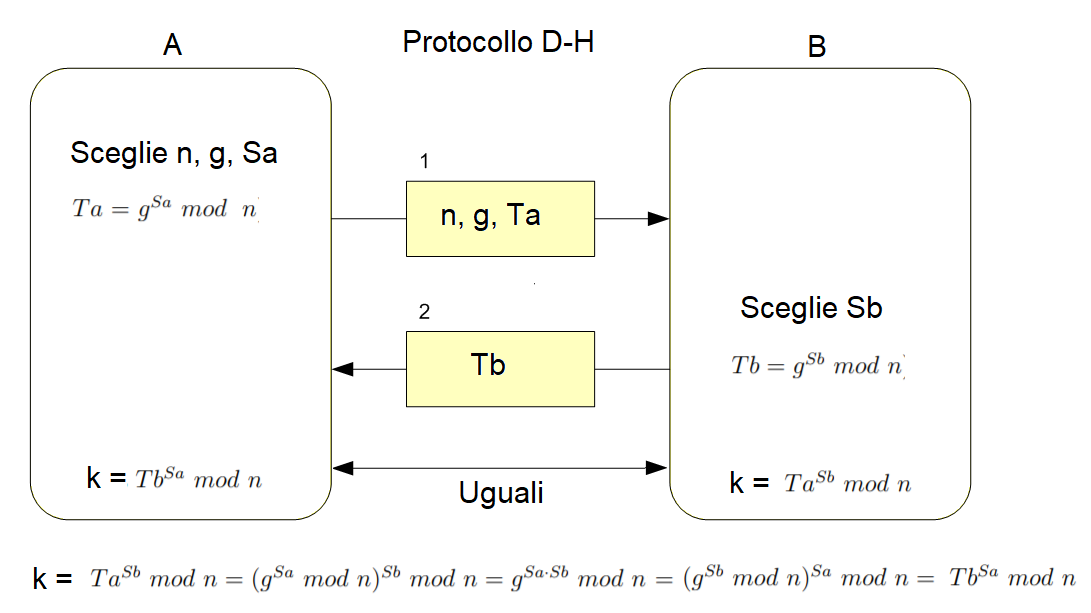
\includegraphics[width=0.8\textwidth]{MainContent/img/cap3/DH.png}
    \caption{Protocollo Diffie Hellman}
    \label{fig:DH}
\end{figure}
\begin{esempio} \\
    Con numeri semplici:
    \begin{itemize}
        \item A sceglie $n$ = 47, $g$ = 7 e $Sa$ = 10 e manda a B (47, 7, 32) perché $7^{10}$mod 47 = 32;
        \item B sceglie $Sb$ = 6 e manda ad A 8 perché $7^6$mod 47 = 8;
        \item A calcola $(8^{10})$mod 47 = 34;
        \item B calcola $(32^6)$mod 47 = 34;
    \end{itemize}
    A e B usano 34 come chiave segreta condivisa $k$.\\
    Un intruso non può calcolare $Sa$ o $Sb$ anche se intercetta $Ta = g^{Sa}$ $mod$ $n$ o $Tb = g^{Sb}$ $mod$ $n$; non si conosce nessun metodo pratico per effettuare il calcolo.
\end{esempio}
A questo punto i due interlocutori sono entrambi in possesso della chiave segreta e possono cominciare ad usarla per cifrare le comunicazioni successive.
\subsection{Sicurezza del protocollo e considerazioni}
\subsubsection{Intercettazione}
Un attaccante ("eavesdropper") può ascoltare tutto lo scambio DH, rimanendo inosservato. Invece, i protocolli di QKD sono immuni alle intercettazioni da parte di terzi, poiché i due interlocutori verrebbero a conoscenza dell'accaduto e scarterebbero le informazioni appena trasmesse.

\subsubsection{Calcolo della chiave scambiata}
Per calcolare i valori $Sa$, $Sb$, $n$, $g$ utili per calcolare la chiave $ k = g^{Sa \cdot Sb}$ $mod$ $n$, avrebbe bisogno di risolvere il problema del \textbf{logaritmo discreto}, che, come accennato in precedenza, è un processo \textbf{computazionalmente oneroso e richiede parecchio tempo}, in quanto sub-esponenziale (sicuramente molto più del tempo di conversazione tra i 2 interlocutori). Questo, oggi, (utilizzando le tecnologie tradizionali) è considerato un problema \textbf{difficile}. \\
\cite{kong_review_2022}
Con l'avvento delle tecnologie quantiche, però, non ci sono prove teoriche che lo schema Diffie-Hellman possa proteggere incondizionatamente la chiave segreta da un intercettatore con risorse quantistiche illimitate. Infatti è stato dimostrato che un computer quantistico risolve il problema del logaritmo discreto in un lasso di tempo sostanzialmente inferiore a quello impiegato da un calcolatore comune. Di conseguenza, essere in grado di calcolare in modo efficiente logaritmi discreti implica essere in grado di rompere Diffie-Hellman, il quale risulta totalmente insicuro contro un avversario che possiede tecnologie quantistiche arbitrarie. Sebbene la crittografia post-quantica possa essere utilizzata per rafforzare lo schema Diffie-Hellman, in questa relazione mi vorrei soffermare sulle tecnologie di Quantum Key Distribution, che proteggono la chiave segreta attraverso i fondamenti della fisica. Le tecnologie quantistiche trattate risolvono questo problema a monte, ovvero un attaccante viene rilevato dalle controparti non appena tenta di intercettare le informazioni scambiate attraverso il canale quantistico. L'unico attacco possibile è quello a forza bruta ma, siccome ogni chiave viene utilizzata una volta soltanto (one-time-pad), questo è poco efficace. Inoltre, i protocolli QKD non dipendono dalla complessità computazionale e, quindi, non sono a rischio di diventare obsoleti di fronte al rapido sviluppo della potenza di calcolo. \\

\subsubsection{Man in the middle}
L'algoritmo Diffie-Hellman è vulnerabile all'attacco "Man in the middle", durante il quale un agente terzo può falsificare le chiavi pubbliche di Alice e Bob ed ingannare le due parti. L'algoritmo DH infatti attua lo scambio delle chiavi simmetriche segrete, ma con il presupposto di avere delle informazioni pubbliche condivise e si dimostra resistente nei confronti dell'intercettamento di queste ultime (a partire dalle informazioni pubbliche non si riesce a ricostruire la chiave, è computazionalmente difficile). Ma nulla può impedire che le informazioni pubbliche siano state modificate o falsificate; in questo caso Alice e Bob non avrebbero modo di accorgersi della frode appoggiandosi al solo algoritmo Diffie-Hellman. Ecco perché occorre che le informazioni pubbliche, ovvero gli elementi $n, g$, possano essere autenticate tramite un algoritmo di autenticazione o da un'autorità di certificazione (CA).
In questo caso, anche i protocolli di QKD sono vulnerabili a questo tipo di attacco ed è necessario che le due parti si autentichino a vicenda per poi stabilire una connessione sicura.

\subsubsection{Forward Secrecy}
Il protocollo Diffie-Hellman è stato progettato per offrire FS, difatti ogni chiave effimera derivata è \textbf{indipendente}. Tanto è vero che, se un attaccante dovesse ricavarne una, sarà in grado di decifrare solamente la relativa conversazione ed esso non avrebbe alcuna informazione sulle altre chiavi. Questo è vero anche per il protocollo di QKD BB84.

\subsubsection{Comparazione Diffie-Hellman e Quantum Key Distribution}
\begin{table}[H]
\centering
    \begin{tabular}{|c|c|c|}
    \hline
     & D-H & QKD\\
    \hline
    Intercettazione & Vulnerabile & \makecell{Sicuro: Le due parti possono verificare \\la presenza di un intercettatore}\\
    \hline
    \makecell{Calcolo della\\chiave  condivisa}& \makecell{Vulnerabile\\(con tecnologie quantistiche)} & \makecell{Sicuro: l'unico attacco possibile è\\ l'attacco a forza bruta ma la chiave\\ viene cambiata continuamente}\\
    \hline
    \makecell{Man in the middle} & Vulnerabile & Vulnerabile\\
    \hline
    \makecell{Forward Secrecy} & Garantita & Garantita\\
    \hline
    \end{tabular}
    \caption{Comparazione tra DH e QKD}
    \label{tab:DH_vs_QKD}
\end{table}
\newpage
\section{Scambio di chiavi con RSA}
Un altro protocollo utilizzato per lo scambio di chiavi effimere è il protocollo asimmetrico RSA (Rivest–Shamir–Adleman) \cite{noauthor_rsa_2022}. RSA è basato sull'elevata complessità computazionale della fattorizzazione in numeri primi. Il suo funzionamento base è il seguente:
\begin{enumerate}
    \item si scelgono a caso due numeri primi, $p$ e $q$ abbastanza grandi da garantire la sicurezza dell'algoritmo (ad esempio, il più grande numero RSA, RSA-2048, utilizza due numeri primi lunghi più di 300 cifre).
    \item si calcola il loro prodotto $n = pq$, chiamato modulo (dato che tutta l'aritmetica seguente è modulo $n$), e il prodotto $\varphi(n)=(p-1)(q-1)$, dove
    $\varphi(n)$ è la funzione toziente.
    \item si considera che la fattorizzazione di $n$ è segreta e solo chi sceglie i due numeri primi, $p$ e $q$, la conosce.
    \item si sceglie poi un numero $e$ (chiamato esponente pubblico), coprimo con $\varphi(n)$ e più piccolo di $\varphi(n)$.
    \item si calcola il numero $d$ (chiamato esponente privato) tale che il suo prodotto con $e$ sia congruo a $1$ $mod$ $\varphi(n)$ ovvero che $ed$ $\equiv$ $1$ $mod$ $(\varphi (n))$
\end{enumerate}
La chiave pubblica è $K_{pub} = (n,e)$, mentre la chiave privata è $K_{priv}(n,d)$.
La forza dell'algoritmo sta nel fatto che per calcolare $d$ da $e$ (o viceversa) non basta la conoscenza di $n$ ma serve il numero $\varphi(n)=(p-1)(q-1)$, e che il suo calcolo richiede tempi molto elevati; infatti fattorizzare in numeri primi (cioè scomporre un numero nei suoi divisori primi) è un'operazione computazionalmente molto costosa.\\
Se Alice e Bob sono in possesso delle chiavi pubbliche dell'altro e, se volessero scambiarsi una chiave effimera segreta, il procedimento è il seguente:
\begin{enumerate}
    \item Alice genera una chiave $k$ (con generatori casuali o scelta da lei) da utilizzare in seguito come chiave simmetrica.
    \item Alice la cifra utilizzando la chiave pubblica di Bob $K_{pubB}= (e,n)$, quindi calcola il valore $c = k^e$ $mod$ $n$ e lo invia a Bob.
    \item Bob utilizza la propria chiave privata $K_{privB}= (d,n)$ per decifrare il messaggio ricevuto da Alice, quindi calcola $c^d$ $mod$ $n$ $=$ $k^{ed}$ $mod$ $n$ $=$ $k^1\;mod\;n$ $=$ $k$
\end{enumerate}
A questo punto i due interlocutori sono entrambi in possesso della chiave segreta $k$ e possono cominciare ad usarla per cifrare le comunicazioni successive.

\subsection{Sicurezza del protocollo e considerazioni}
\subsubsection{Intercettazione}
Un attaccante ("eavesdropper") può ascoltare lo scambio, ma per calcolare la chiave condivisa $k$ deve decifrare il messaggio criptato, ovvero trovare i fattori primi di $n$. Come annunciato in precedenza, questo è un calcolo incredibilmente complesso per i calcolatori comuni. Tuttavia, è stato dimostrato che l'algoritmo di \textbf{Shor} \cite{shor_polynomial-time_1997} permette di scomporre il numero $n$ nei suoi fattori primi $p$ e $q$ in tempo \textbf{polinomiale} (cioè sub-esponenziale). In questo modo, se l'attaccante avesse a disposizione risorse quantistiche arbitrarie, sarebbe in grado di "rompere" l'algoritmo RSA e di ricavare la chiave segreta scambiata tra i due interlocutori.
\subsubsection{Man in the middle}
Anche in questo caso, l'unico attacco attivo che si può pensare è il man-in-the-middle, cioè c'è la possibilità che l'attaccante si inserisca nelle comunicazioni tra Alice e Bob nel momento dello scambio delle chiavi pubbliche: questo accade perché le chiavi, di per sé, non sono autenticate. In TLS vengono utilizzati i certificati digitali a questo scopo.
\subsubsection{Osservazioni temporali o timing attack}
Si tratta di un attacco insolito ed nessuno se lo sarebbe mai aspettato quando fu standardizzato il protocollo. Si tratta, di fatto, di analizzare quanto tempo ci mette un algoritmo a decifrare una messaggio \cite{timing_attack}. Esiste, infatti, una stretta correlazione tra la chiave privata e la difficoltà computazionale richiesta per cifratura e decifratura: basta osservare quanto tempo serve ad un algoritmo per decifrare un messaggio (con la chiave pubblica) per avere alcune informazioni sulla chiave privata. Per ovviare a questo problema, le implementazioni commerciali di RSA, ad oggi, inseriscono delle attese casuali nel software, in modo da annullare la correlazione tra la firma ed il tempo necessario per decifrare i messaggi. I protocolli di QKD non sono soggetti a questo problema.
\subsubsection{Forward Secrecy}
Quando in TLS viene utilizzato RSA (e non Diffie-Hellman) per lo scambio di chiavi, per un attaccante è sufficiente ottenere la chiave privata del server per decriptare tutte le sessioni (passate e future) avviate con quel server e di conseguenza è possibile ricavare tutte le chiavi effimere scambiate tra le due parti. In sostanza, ricavando una chiave effimera l'attaccante sarà in grado di ottenere \textbf{tutte} le altre, in quanto non sono "indipendenti" (a differenza di DH). Infatti è noto come lo scambio di chiavi basato su RSA \textbf{non offra} la \textbf{forward secrecy}, ovvero la proprietà che assicura che se una chiave di cifratura a lungo termine viene compromessa, le chiavi di sessione generate a partire da essa rimangono riservate.
Questa tecnica viene attuata, ad esempio, utilizzando il popolare sniffer di rete Wireshark per ispezionare le connessioni protette da TLS.
Questo problema può essere risolto sostituendo il meccanismo RSA con il protocollo di QKD affiancato da OTP. In questo modo, nel caso in cui un eventuale attaccante dovesse in ottenere una delle chiavi effimere, sarà in grado di decifrare solamente una porzione ridotta dei messaggi scambiati, poiché le chiavi vengono cambiate di continuo (One Time Pad).

\subsubsection{Comparazione RSA e Quantum Key Distribution}
\begin{table}[H]
\centering
    \begin{tabular}{|c|c|c|}
    \hline
     & RSA & QKD\\
    \hline
    Intercettazione & Vulnerabile & \makecell{Sicuro: Le due parti possono verificare \\la presenza di un intercettatore}\\
    \hline
    \makecell{Calcolo della\\chiave  condivisa}& \makecell{Vulnerabile\\(con tecnologie quantistiche)} & \makecell{Sicuro: l'unico attacco possibile è\\ l'attacco a forza bruta ma la chiave\\ viene cambiata continuamente}\\
    \hline
    \makecell{Man in the middle} & Vulnerabile & Vulnerabile\\
    \hline
    \makecell{Timing attack} & Vulnerabile & Sicuro\\
    \hline
    \makecell{Forward Secrecy} & Non garantita & Garantita\\
    \hline
    \end{tabular}
    \caption{Comparazione tra RSA e QKD}
    \label{tab:RSA_vs_QKD}
\end{table}
\chapter{Quantum Key Distribution in TLS}
Il protocollo TLS è stato sviluppato da Netscape \cite{freier_secure_2011} e standardizzato successivamente da IETF \cite{rescorla_transport_2008}. È un protocollo standard di sicurezza che permette connessioni sicure tra due entità comunicanti, fornendo autenticazione, integrità dei dati e confidenzialità. TLS è composto da cinque protocolli minori: Record Protocol, Handshake Protocol, Change Spec Protocol, Alert Protocol e Application Data Protocol \cite{elboukhari_improving_nodate}.

\section{QKD in TLS Hanshake Protocol}
Il protocollo TLS Record utilizza il protocollo TLS Handshake per generare parametri di sicurezza, in cui è incluso il processo di distribuzione delle chiavi. Nella descrizione di TLS Handshake \cite{rescorla_transport_2008} la distribuzione delle chiavi è limitata al solo protocollo di scambio Diffie Hellman (DH) e RSA. Il problema è che, come discusso in precedenza, sia DH che RSA non sono incondizionatamente sicuri, infatti la loro sicurezza dipende dalla potenza di calcolo o dal tempo necessario per calcolare le chiavi. Utilizzando la Quantum Key Distribution, la sicurezza del protocollo è indipendente dalla quantità di risorse possedute dall'attaccante e di conseguenza questa non sarà minacciata dal progresso tecnologico. Per questo motivo si è pensato di integrare QKD nel Protocollo TLS al posto dello scambio di chiavi DH o RSA \cite{elboukhari_improving_nodate}.

\subsection{Requisiti per l'implementazione}
Per integrare QKD nel protocollo TLS alcuni requisiti devono essere soddisfatti:
\begin{itemize}
    \item Un canale ottico: QKD utilizza i fotoni per codificare le informazioni. Ci sono due mezzi per trasportare i fotoni: la fibra ottica o lo spazio libero \cite{hughes_practical_2002}. La fibra riduce di molto i rumori rispetto all'aria libera ed infatti è la più utilizzata nei sistemi quantistici.
    
    \item Modem ottico: il modem può svolgere il ruolo di ricevitore ed emettitore di fotoni. Il modem dovrebbe anche includere un polarizzatore per codificare i dati utilizzando diverse basi di polarizzazione. Viene utilizzato per scambiare la chiave quantistica, ma può anche essere utilizzato per inviare dati comuni a seconda del metodo di codifica delle informazioni. Il modem è molto importante poichè può recitare entrambi i ruoli, di canale quantistico e di canale classico. Esistono alcune implementazioni di tale dispositivo \cite{thesis}.
    
    \item Protocollo di QKD: per generare una chiave e scambiarla è necessario implementare un protocollo di QKD tra i due modem ottici. La chiave una volta generata, viene archiviata in una memoria flash per essere utilizzata nella fase di cifratura dei dati. Il protocollo più comune è BB84, il quale si è dimostrato sicuro e semplice da implementare.
\end{itemize}

\subsection{QKD Configuration Protocol}
Nell’obiettivo di ideare un nuovo schema di TLS che possa includere il servizio di QKD, è stato introdotto un componente addizionale, il QKD Configuration Protocol, che permette di configurare i parametri necessari per lo scambio QKD. Quindi il nuovo protocollo TLS avrà cinque componenti: i classici protocolli handshake, Change Spec, Alert, Application e in aggiunta il \textbf{QKD Configuration}. Il formato del messaggio del protocollo di configurazione QKD contiene i seguenti campi:

\begin{itemize}
    \item Type (1 byte): indica il tipo di protocollo di crittografia quantistica utilizzato. Ad esempio protocolli basati sul principio di indeterminazione di Heisenberg come BB84 o protocolli basati sulla disuguaglianza di Bell come E91.
    
    \item Protocollo (1 byte): indica il protocollo utilizzato (ad es. BB84, B92 o E91).
    
    \item Versione (1 byte): consente l'utilizzo di più versioni dello stesso protocollo.
    
    \item Lunghezza (4 byte): indica la lunghezza del messaggio in byte.
    
    \item Key-Length (4 byte): mostra la lunghezza della chiave ottenuta dal protocollo di QKD. La sua lunghezza varia da 1 a 4 byte. Scegliamo la lunghezza molto grande in modo da usare \textit{One-Time-Pad} per ottenere sicurezza incondizionata. In questo caso la lunghezza della chiave deve essere uguale alla lunghezza dei dati da codificare \cite{shannon_communication_1949}.
    
    \item TTL field (2 byte meno un bit): indica, in termini di tempo (in secondi) o il numero di messaggi in cui una chiave potrebbe essere usata nel processo di codifica. Una volta che il tempo è finito o il numero massimo di messaggi è stato raggiunto, il meccanismo di QKD provvede a generare una nuova chiave.
    
    \item T field (1 bit): questo campo specifica se consideriamo il tempo o il numero di messaggi in cui la chiave può essere usata nel processo di codifica. Quando il valore è 1, il campo TTL mostra l’ammontare di tempo, quando invece il valore `e 0, il campo TTL corrisponde al numero di messaggi.
    
    \item Autenticazione (1 byte): mostra se il messaggio è autenticato o meno.
    
    \item Codifica (1 byte): questo campo specifica una determinata tecnica di codifica se utilizzata per crittografare il contenuto del messaggio.
    
    \item Contenuto (la sua lunghezza non è fissa)
\end{itemize}

\begin{figure}[H]
    \centering
    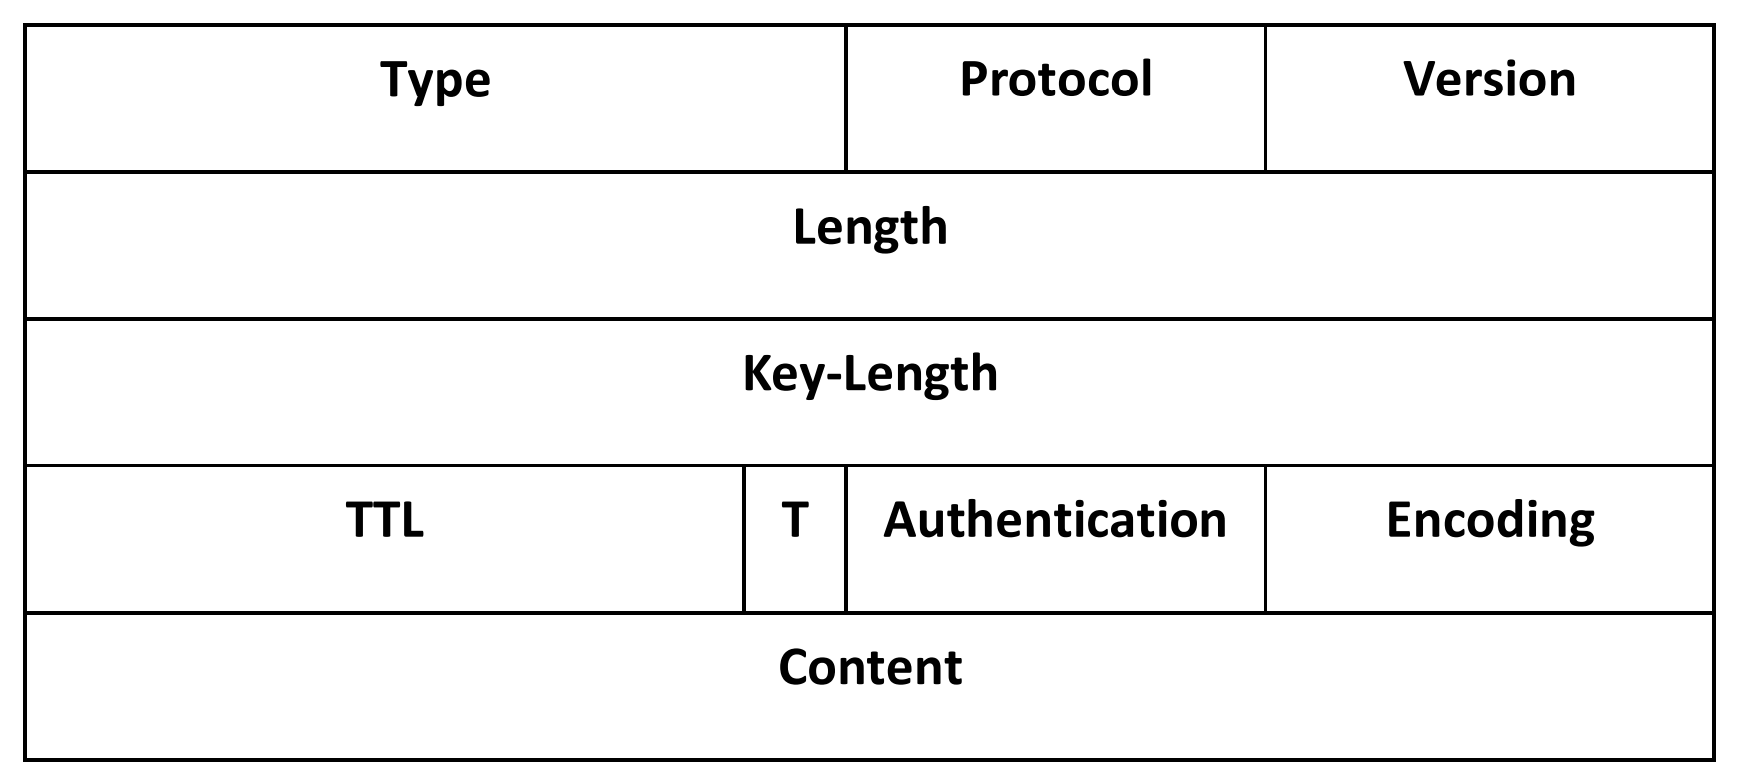
\includegraphics[width=0.8\textwidth]{MainContent/img/cap3/QKD Configuration Protocol.png}
    \caption{Formato messaggi di QKD Configuration Protocol}
    \label{fig:QKD_conf}
\end{figure}

\subsection{Quantum TLS Handshake Protocol}
Nello schema di TLS sono state introdotte alcune modifiche al protocollo di Handshake, in particolare la procedura classica di scambio delle chiavi (DH, RSA) è stata sostituita con il meccanismo di QKD utilizzando il protocollo BB84. Per questo motivo, verrà rinominato \textbf{Quantum TLS Handshake} . La Figura sottostante mostra i diversi messaggi inviati in questo protocollo.
\begin{figure}[H]
    \centering
    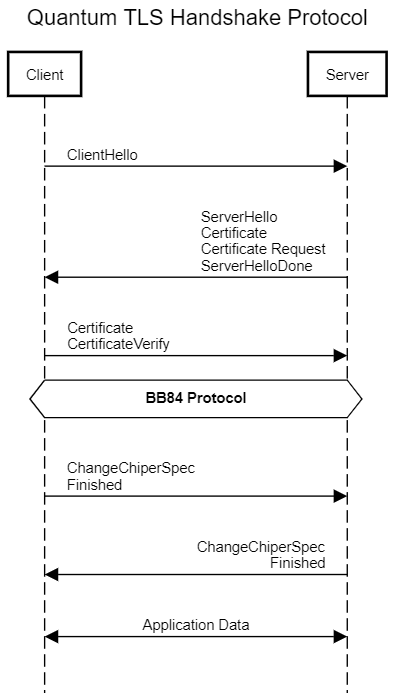
\includegraphics[width=0.5\textwidth]{MainContent/img/cap3/BB84diagram.png}
    \caption{Quantum TLS Handshake Protocol}
    \label{fig:QTLSHP}
\end{figure}
\noindent È possibile notare come il protocollo quantico BB84 sia integrato nell'handshake TLS. Inizialmente è presente una fase di autenticazione, in cui il Client ed il Server si autenticano reciprocamente scambiandosi i certificati. Una volta conclusa questa fase, viene eseguito il protocollo quantico ed il numero di fotoni che deve essere trasmesso dipende dalla lunghezza della chiave desiderata. Siccome BB84 è vulnerabile agli attacchi di tipo man-in-the-middle, una volta finita l’esecuzione del processo viene verificato se l’autenticazione è andata a buon fine.
\newpage

\subsection{Esempio di applicazione di questa soluzione QKD-TLS}
Per dimostrare l'effettiva applicabilità di questa soluzione, in questa sezione è presentato un esempio di implementazione di QKD-TLS \cite{laurenti_integration_nodate}. Consideriamo due reti LAN connesse da due modem ottici che giocano il ruolo di canale quantico e classico
allo stesso tempo. Il processo che permette di assicurare la sicurezza della connessione TLS tra Alice e Bob utilizzando il meccanismo di QKD è composto da cinque fasi:
\begin{figure}[H]
    \centering
    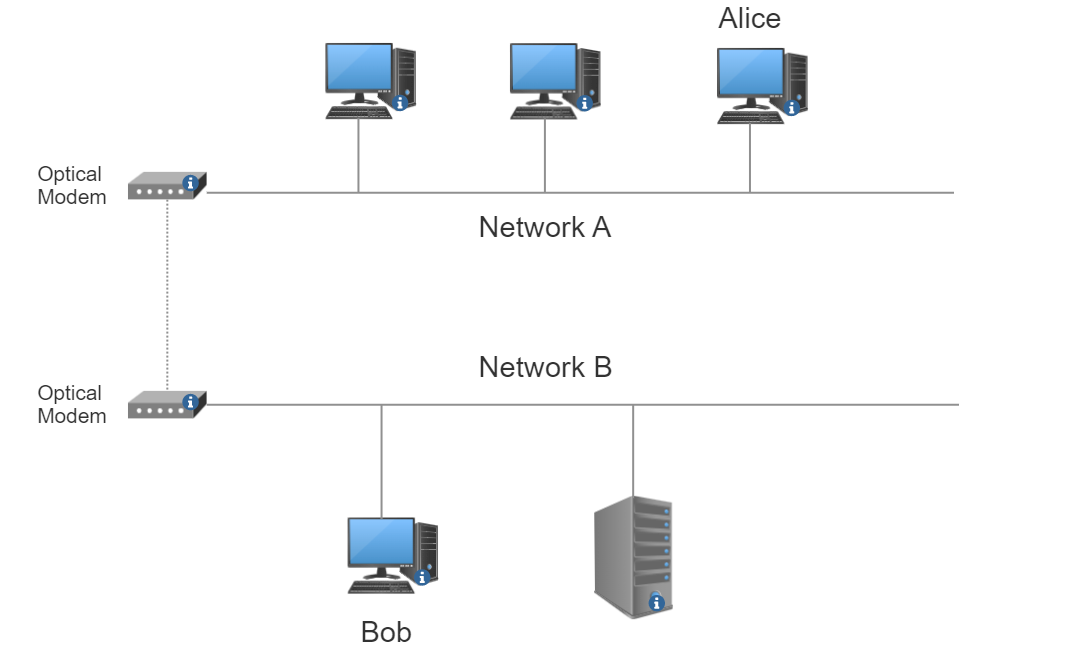
\includegraphics[width=0.8\textwidth]{MainContent/img/cap3/EsempioTLS.png}
    \caption{Esempio d’uso di due modem ottici in Quantum TLS}
    \label{fig:esempio}
\end{figure}

\begin{itemize}
    \item \textbf{Fase 1}: quando il TLS Record Protocol del nodo A, per esempio, prende i dati dal livello di applicazione, chiama il suo Application Data Protocol. Così i dati sono frammentati e per ogni frammento viene fatta una compressione.
    \item \textbf{Fase 2}: il TLS record Protocol chiama il QKD Configuration Protocol in modo che i nodi A e B si mettano d’accordo sui parametri del QKD Configuration Protocol illustrati in precedenza. I campi più importanti sono: \textit{protocol}, \textit{key - length} e i campi \textit{TTL} e \textit{T}. Nell’esempio scegliamo il protocollo BB84 perchè è il primo protocollo sperimentato ed è provata la sua sicurezza incondizionata. Assumiamo che non vi siano meccanismi di autenticazione e di codifica. Prendiamo in considerazione: \textit{Key - length} = 20 byte, \textit{TTL} = 200 messaggi, \textit{T} = 0. Nel caso in cui si volessimo utilizzare one-time-pad, per testare la sicurezza incondizionata dobbiamo scegliere \textit{TTL} = 1.
    
    \item \textbf{Fase 3}:  Il TLS Record Protocol usa il Quantum Handshake Protocol per ottenere i parametri di sicurezza. Così il Quantum Handshake Protocol viene eseguito e viene attuato il protocollo BB84 nei due modem. La chiave generata viene memorizzata in una memoria flash per essere usata più tardi nella codifica dal Record Protocol.
    
    \item \textbf{Fase 4}:Il TLS Record Protocol riceve la chiave fornita dal servizio QKD e costruisce i suoi parametri di sicurezza. Questi parametri sono usati per generare chiavi per codificare dati e assicurare l’integrità (MAC).
    
    \item \textbf{Fase 5}: una volta che il record (frammenti compressi, MAC e pudding opzionale) è stato criptato, al blocco appena codificato viene aggiunto un header e l’intero pacchetto viene passato al livello di trasporto.
\end{itemize}








\include{MainContent/capitolo5}
\chapter*{Conclusione}
In questa relazione ho analizzato la tecnologia della Quantum Key Distribution, descrivendo i protocolli più famosi e le loro caratteristiche. Sono stati evidenziati i punti di forza e debolezza di questa nuova tecnologia, in modo tale da avere una visione più ampia dell'argomento. Abbiamo visto quindi che uno dei più grandi benefici della QKD `e quello di generare e distribuire chiavi sicure attraverso canali non sicuri. Ci sono però ancora delle limitazioni come il costo della tecnologia o il fatto che la QKD richiede un hardware dedicato.. È stata posta particolare attenzione a due protocolli crittografici che permettono lo scambio di chiavi, DH e RSA, grazie ai quali è stato possibile effettuare confronti per quanto riguarda la sicurezza di QKD. È stato possibile osservare che sia DH che RSA possiedono vulnerabilità sfruttabili con opportune risorse quantistiche e che l'utilizzo di QKD potrebbe mitigare alcuni possibili attacchi. Infine, ho mostrato un esempio di come questa tecnologia possa essere implementata nel protocollo TLS (nello specifico nell'Handshake TLS), in modo tale da aumentare la sicurezza e la segretezza delle comunicazioni. È necessario sottolineare però che l'utilizzo di protocolli di QKD comporta diverse problematiche, le quali non possono essere trascurate. La QKD è una tecnologia ancora in fase sperimentale e sicuramente grazie agli sviluppi futuri sarà possibile determinare l'effettiva validità ed efficacia di questa soluzione

\addcontentsline{toc}{chapter}{Conclusione}

\end{spacing}

\nocite{*}
\bibliographystyle{ieeetr}
\bibliography{mybib}
\end{document}